\section{Software Design Process}
\label{sec:design}

The software design process has been inspired by the Use Case 2.0 \cite{jacobson2011usecase} of Iva Jacobsen \textit{et al.}. This approach is an extension of the \gls{UML} definition for \glspl{use_case} and includes a more specific approach how to deal with different layers of abstraction. This helps to guide the requirement analysis in an efficient way and enables easy communication between software engineers and non-coders. A brief overview of the used approach can be found in \autoref{fig:usecase20:flow}.

\begin{figure}[!ht]
\centering
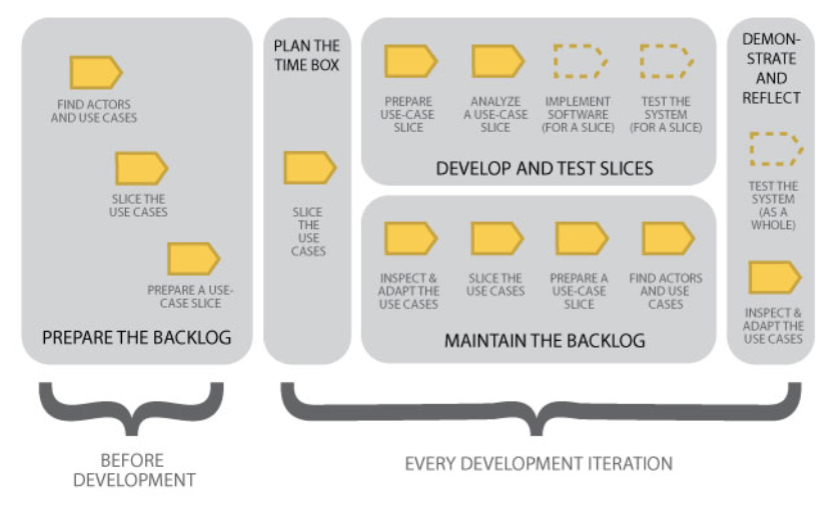
\includegraphics[width=0.8\textwidth]{figures/uc20_flow}
\caption{\gls{use_case} 2.0 activities for iterative development approaches \cite{jacobson2011usecase}}
\label{fig:usecase20:flow}
\end{figure}


\subsection{Use-Cases, Use-Case Flows and Use-Case Slices}
Use cases are the core concept in Use Case 2.0. In addition to the \gls{UML} specification \glspl{use_case} are described as cards including the attributes Priority, Release, Size and Complexity. For the prioritisation the MoSCoW\todo{reference} (Must, Should, Could, Would) is used. After the initial requirement analysis, \glspl{use_case_slice} are generated usually including flows, tests and an estimation of the development. In this step the different \glspl{Actor} are identified and test cases are defined. To do so, the \glspl{use_case_slice} are analysed to check how the system elements will interact to perform the assigned \gls{use_case}. The \glspl{use_case_slice} are then going to be implemented and tested with the previous defined test scenarios. Finally the whole system will be tested with \glspl{e2e_test}.

\textbf{\glspl{use_case}} are the general tasks the system and the actors will perform. They are big, not thought completely through and do not contain directly implementable tasks.

\textbf{\glspl{use_case_flow}} are the different flows, how the interaction between actors and the system take place. Usually there is a standard flow, and alternative (error / exception handling) flows. These will be specified later when we go deeper into the analysis. In the state of Use Case Flows we will as well generate Test Cases for the flows. 

\textbf{\glspl{use_case_slice}} are the final development tasks. They will be generated out of the Use Case Flows and can be independently implemented as a single iteration step. They are bases on the Flows and Test Cases. Further Test Cases are usually generated during the implementation react on system specific scenarios.


\subsection{Test Driven development}
\label{sec:tdd}
\todo{TDD approach}

\subsection{Test Suit}
\label{sub:test_suit}
\todo{Describe test suit}

